\section{Baza XML}

\subsection{Schemat dokumentu}

\begin{figure}[h]
 \centering
 \subfigure[element text]{
 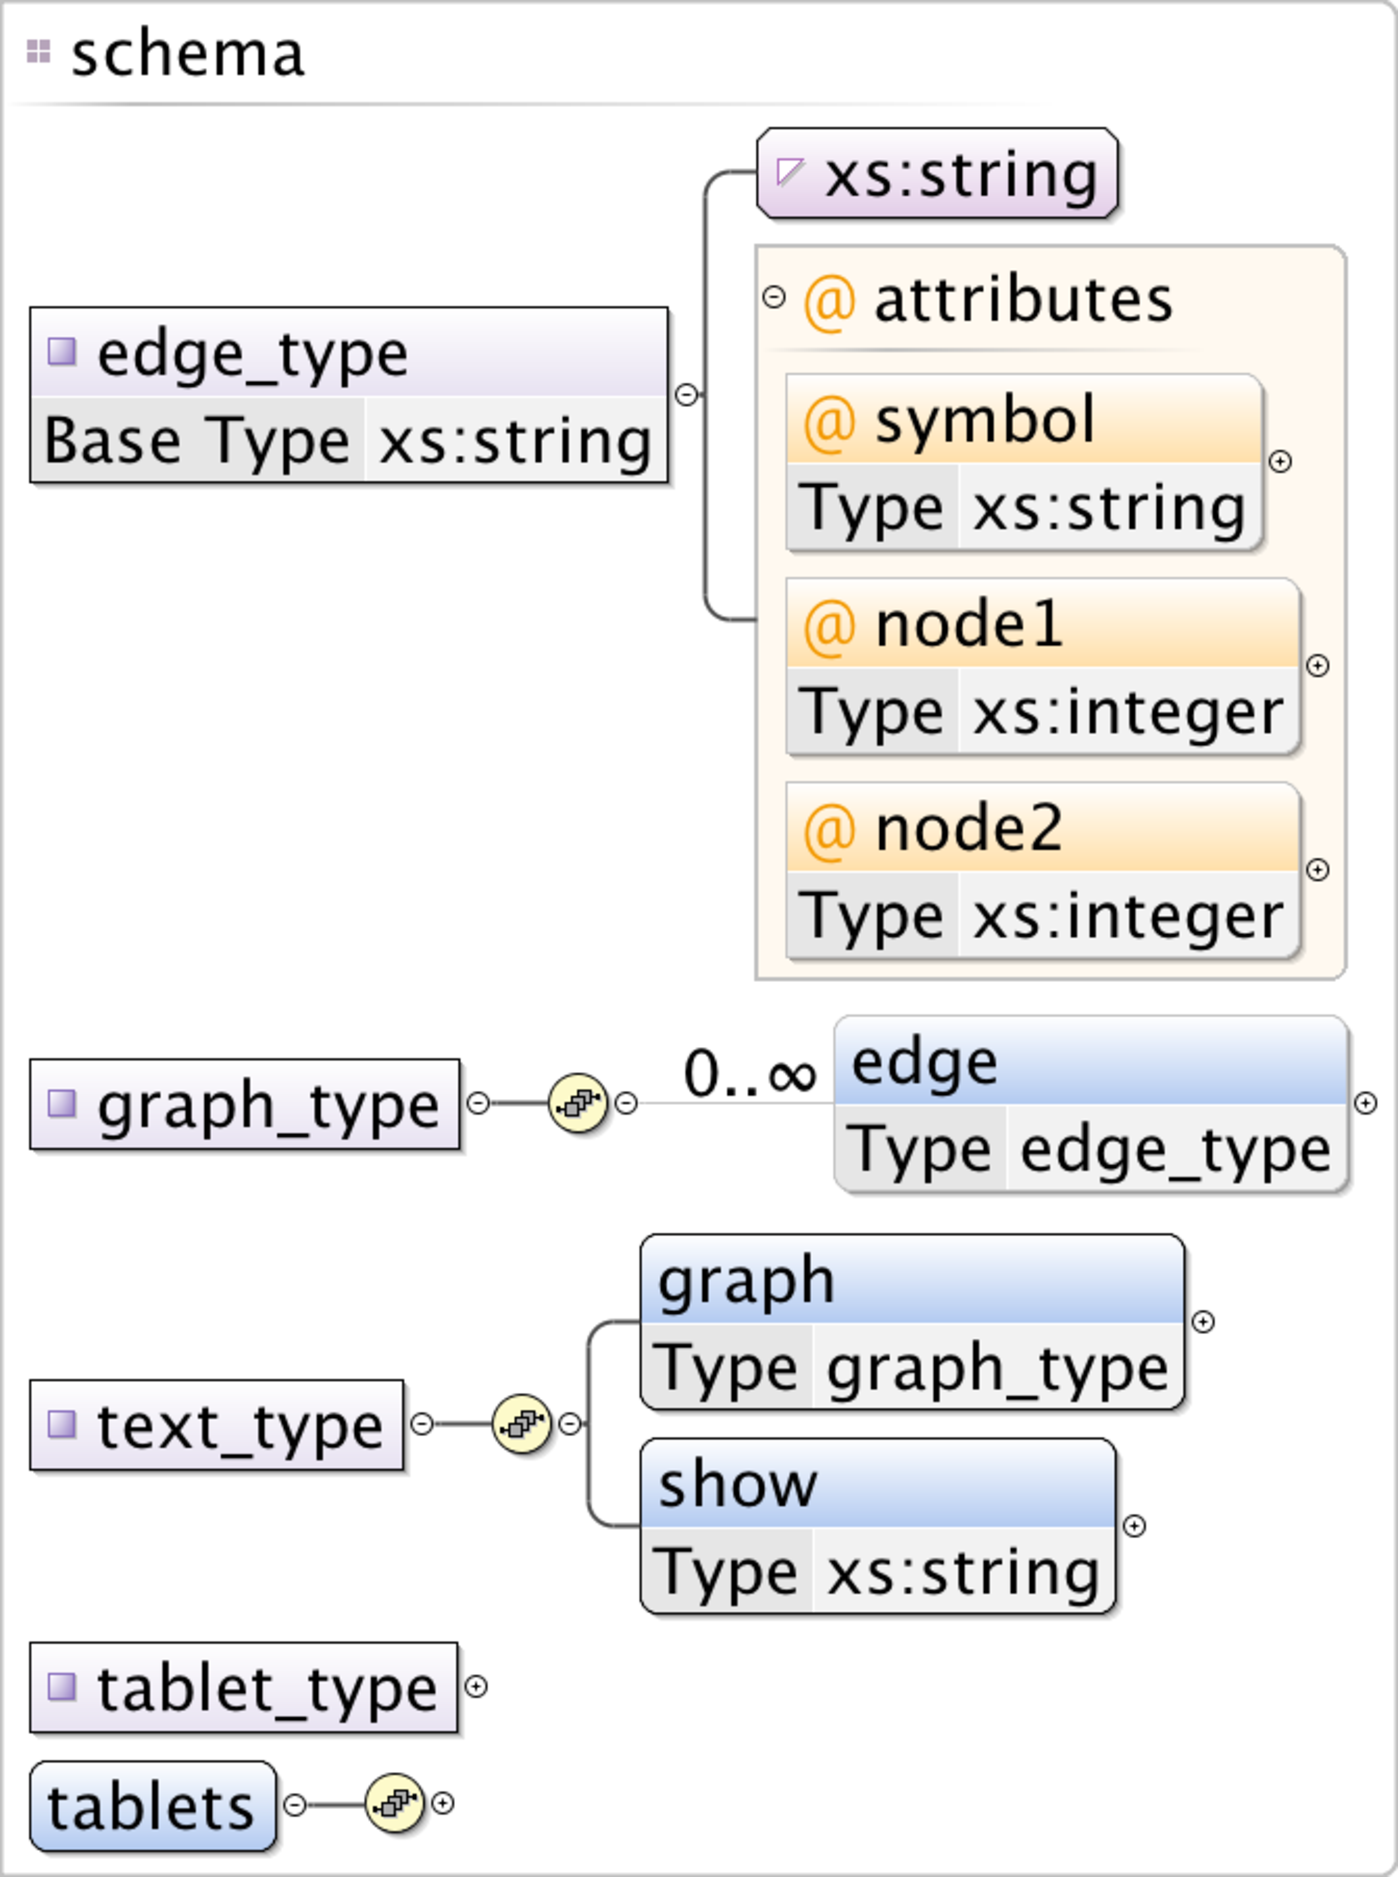
\includegraphics[width=120px]{../diagramy/schema_text.pdf}
 }
   \subfigure[element tablet]{
  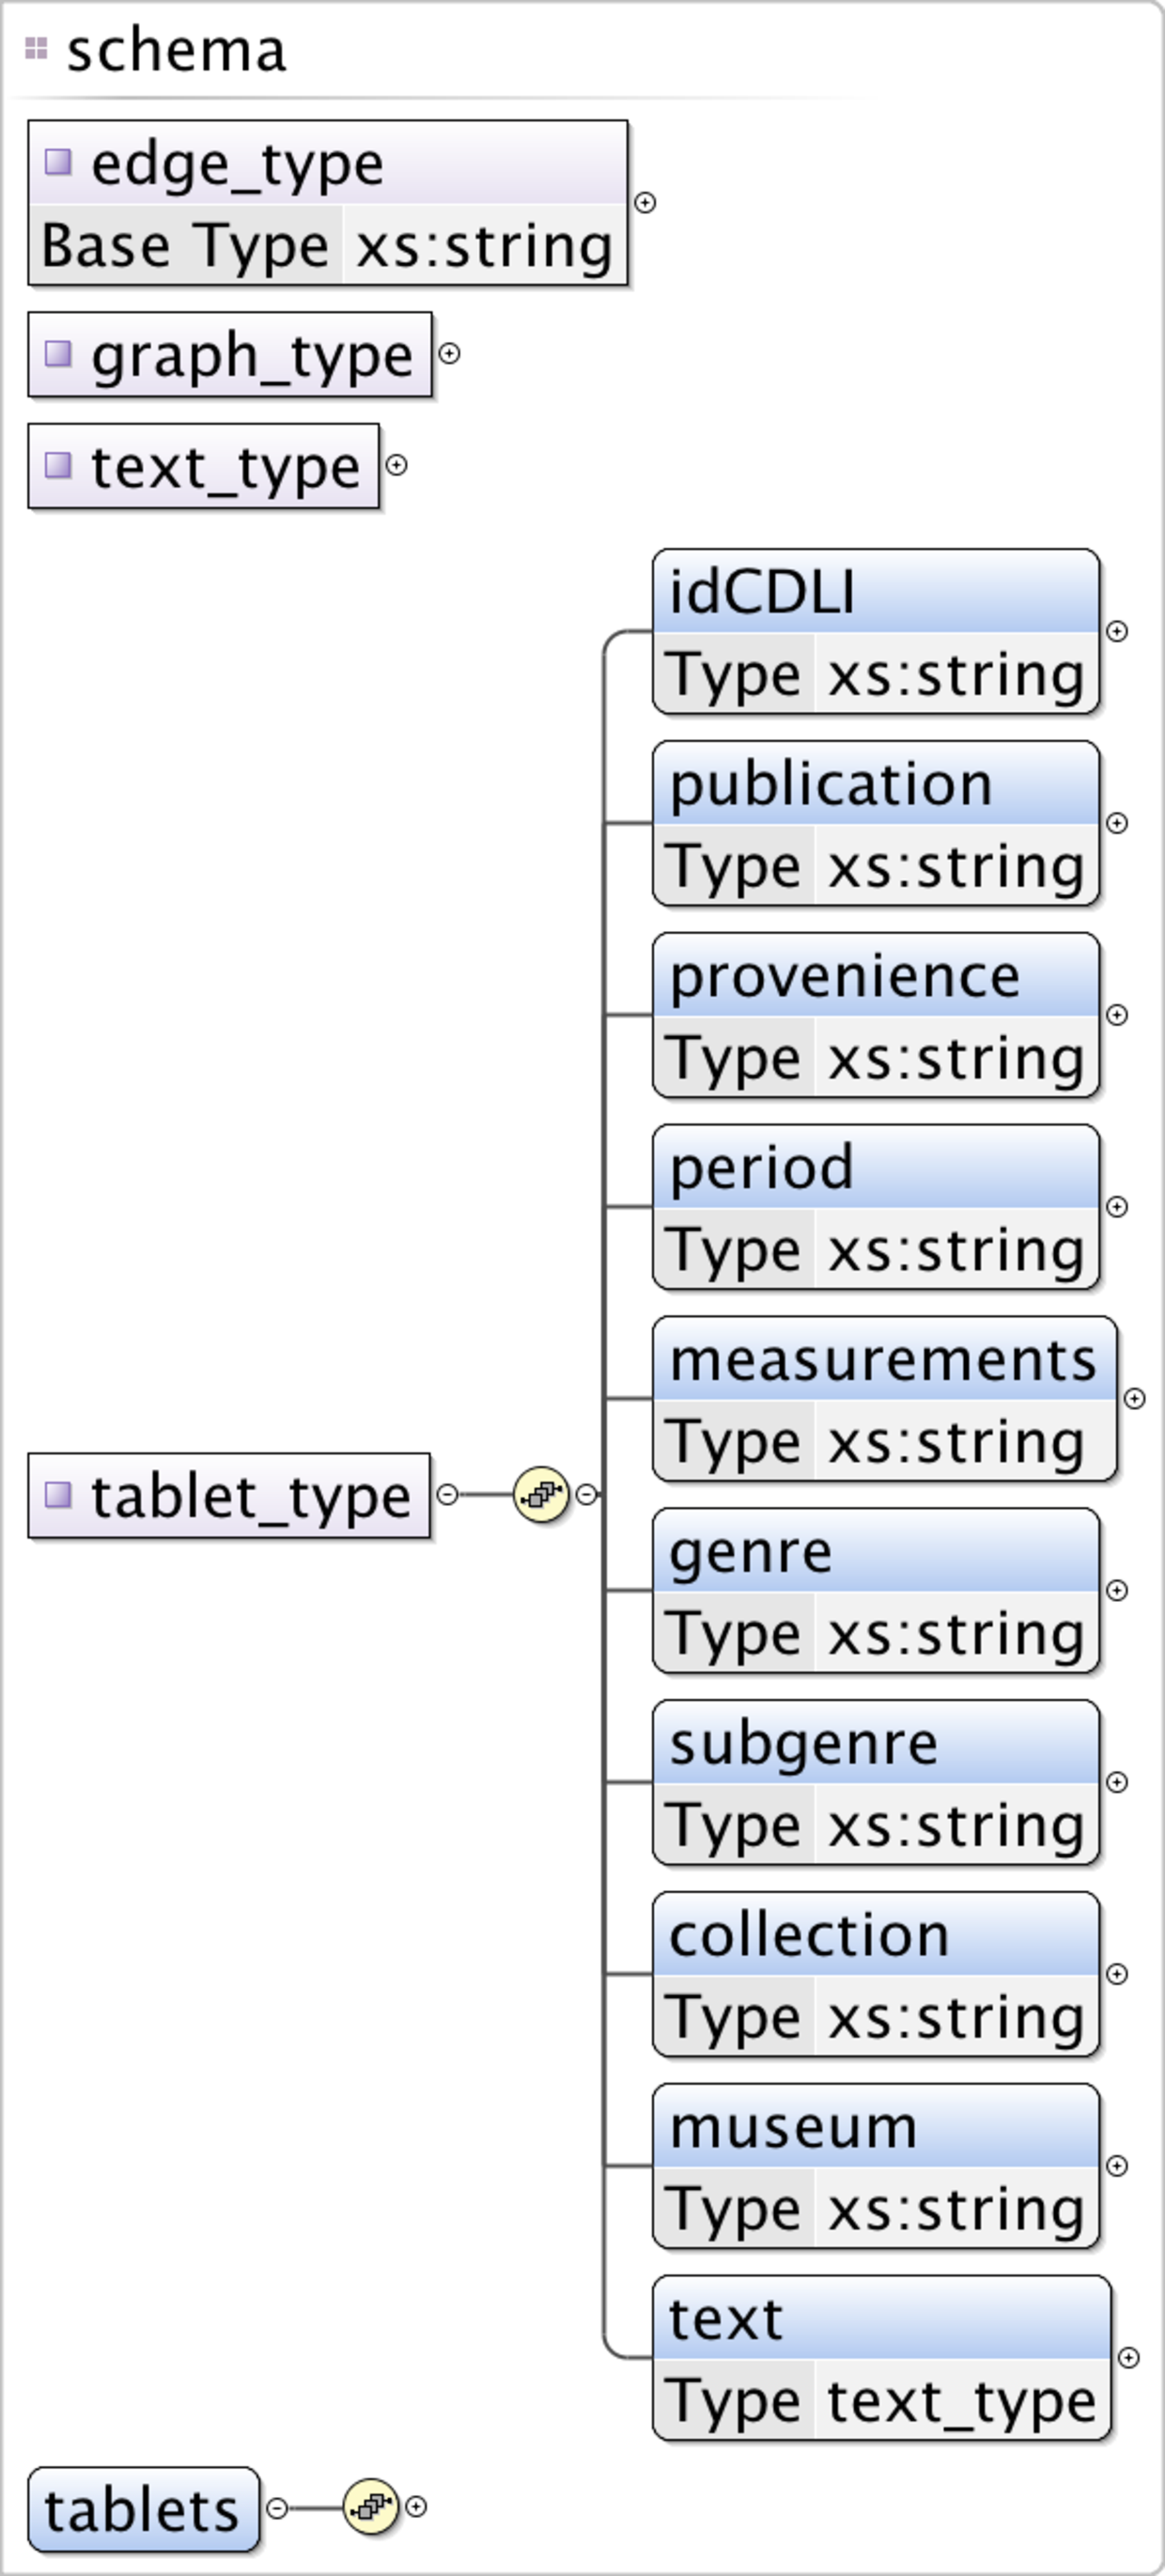
\includegraphics[width=120px]{../diagramy/schema_tablet.pdf}
 }
 \subfigure[element tablets]{
  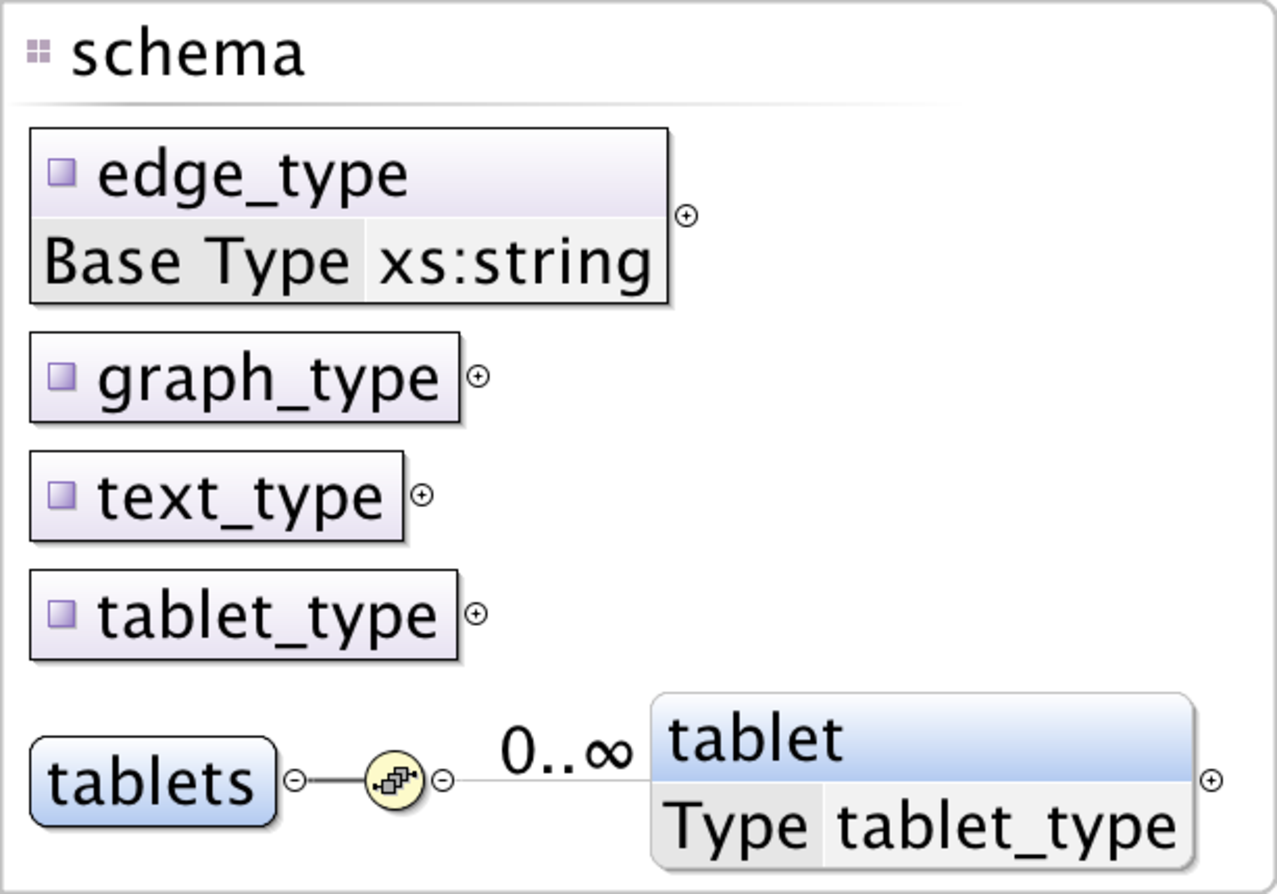
\includegraphics[width=120px]{../diagramy/schema_tablets.pdf}
 }
 \caption{Schematy poszczególnych elementów (kolor pomarańczowy oznacza atrybuty, a niebieski elementy)}
\end{figure}



Schemat dokumentu zamieszczony powyżej jest graficznym przedstawieniem dokumentu XML Schema (dodatek \ref{appendix:xmlsch}) 
wygenerowanym przez program Oxygen.

Przy jego tworzeniu, podobnie jak w bazie relacyjnej, skorzystałyśmy z pomysłu dra Wojciecha Jaworskiego, 
aby przedstawić treść tabliczki w formie grafu. 
Każda krawędź tego grafu (odpowiadająca odczytowi) jest oddzielnym elementem, zawierającym atrybuty \textit{node1}, \textit{node2} 
i \textit{symbol}.
Atrybuty \textit{node1} oraz \textit{node2} oznaczają numery węzłów grafu,
natomiast atrybut \textit{symbol} to typ symbolu znajdującego się na danej krawędzi. 
Dodatkowo przechowujemy treść tabliczki w formie napisu (element \textit{show}). 

Metadane tabliczek przechowywane są w postaci podelementów elementu \textit{tablet}.


\subsection{Translator\_xml}
Do przeszukiwania dokumentu XML wykorzystujemy język XQuery, który jest częścią rekomendacji W3C dotyczącej XML.\\
Proste zapytanie TQL jest tłumaczone na pojedynczą konstrukcję FLWOR (For Let Where Order by Return).\\

\subsubsection{Stałe fragmenty zapytania}
Każde zapytanie w części For zawiera:
	\begin{verbatim}
	FOR $tablet IN .//tablet
\end{verbatim}
a w części Return:
  \begin{verbatim}RETURN <tablet>
		{$tablet/idCDLI}
		{$tablet/publication}
		{$tablet/provenience}
		{$tablet/period}
		{$tablet/measurements}
		{$tablet/genre}
		{$tablet/subgenre}
		{$tablet/collection}
		{$tablet/museum}
		{$tablet/text/show}
		<seq>...</seq>
	</tablet>
\end{verbatim}
Zawartość elementu seq zależy od ilości sekwencji, po których wyszukujemy. 

\subsubsection{Tłumaczenie zapytań o atrybuty tabliczki}

\begin{longtable}{|p{2.5in}|p{3.5in}|}
\hline
{\bf Konstrukcja} & {\bf Tłumaczenie na XQuery}\\
\hline
\endhead
provenience: wartosc & \begin{verbatim}fn:matches($tablet/provenience,'^wartosc$')\end{verbatim}
\\
\hline
publication: wartosc & \begin{verbatim}fn:matches($tablet/publication,'^wartosc$')\end{verbatim}
\\
\hline
period: wartosc & \begin{verbatim}fn:matches($tablet/period,'^wartosc$')\end{verbatim}
\\
\hline
genre: wartosc & \begin{verbatim}(fn:matches($tablet/genre,'^wartosc$')
or fn:matches($tablet/subgenre,'^wartosc$'))\end{verbatim}
\\
\hline
cdli\_id: wartosc & \begin{verbatim}fn:matches($tablet/idCDLI,'^wartosc$')\end{verbatim}
\\
\hline
\end{longtable}


\subsubsection{Tłumaczenie zapytań o treść tabliczki}
Każda sekwencja, po której wyszukujemy powoduje dodanie do zapytania następujących konstrukcji:
\begin{itemize}
\item{do części Let:}
\begin{verbatim}
let $seq <id_sekw> := (
	for $edge_end in $tablet//edge
	for $edge_start in $tablet//edge
	where (
		fn:matches($edge_start,'^<sekw[0]>$')
		and (
			some $edge1 in $tablet//edge[@node1=$edge_start/@node2]
satisfies (fn:matches($edge1,'^<sekw[1]>$')
and ... 
and fn:matches($edge_end,'^<sekw[dl_sekw-1]>$')))))
return <seq<id_sekw>> {$edge_start/@node1} {$edge_end/@node2} </seq<id_sekw>>
\end{verbatim}
\item{do części Where}
\begin{verbatim}
$seq<id_sekw>
\end{verbatim}
\item{do części Return w elemecie seq}
\begin{verbatim}
$seq<id_sekw>
\end{verbatim}
\end{itemize}




\subsubsection{Tłumaczenie operatorów}
Poniższe tłumaczenia dotyczą zarówno konstrukcji prostych jak i złożonych.

\begin{longtable}{|p{1in}|p{3in}|}
\hline
{\bf Operator} & {\bf Tłumaczenie}\\
\hline
\endhead
/ & \begin{verbatim}(<zapytanie1> or <zapytanie2>) \end{verbatim} \\
\hline
-- & \begin{verbatim}not (<zapytanie_negowane>) \end{verbatim}\\  
\hline
+ & \begin{verbatim}(<zapytanie1> and <zapytanie2>) \end{verbatim}\\ 
\hline
* & \begin{verbatim} .*\end{verbatim}  \\ 
\hline
\end{longtable}

\subsubsection{Zapytania złożone}
Zapytanie złożone, składające się z wielu zapytań prostych tłumaczymy na sekwencję zapytań XQuery połączonych znakiem ','.

\subsection{Database\_xml}
Odpowiada za wywołanie zapytania i zapisanie wyniku do struktury Tablets.
Jako bazę danych wykorzystujemy plik XML, określony w pliku konfiguracyjnym xml.conf. 
Do wyszukiwania wykorzystujemy procesor XQuery Zorba. 
Posiada on API m.in. do C++, które pozwala na przekazanie zapytania do bazy oraz przetworzenie wyniku.
